\documentclass{article}
\usepackage[utf8]{inputenc}
\usepackage{graphicx}
\usepackage{chngcntr}
\usepackage{amsthm}
\usepackage{amssymb}
\usepackage{amsmath}

\title{COMP37212 Computer Vision}
\author{Izunna Aneke}
\date{2020}

\graphicspath{{Images/}}

\newtheorem{definition}{Definition}[subsection]
\newtheorem{theorem}{Theorem}[section]
\newtheorem{corollary}{Corollary}[theorem]
\newtheorem{lemma}[theorem]{Lemma}
\newtheorem{example}{Example}[subsection]
\newtheorem*{remark}{Remark}

% Reset equation each time a new section or subsection is entered
\counterwithin*{equation}{section}
\counterwithin*{equation}{subsection}


\begin{document}

\maketitle

\newpage

\tableofcontents

% Make counter also count subsections
\counterwithin{figure}{subsection}

\newpage

\section*{Acknowledgements}
These notes are based on the COMP37212 course from The University of Manchester.

\newpage
\section{Introduction}
\subsection{What is Computer Vision?}
The goal of Computer Vision is to write computer programs that can interpret images.
\\\\
Computer Vision \textbf{interprets visual information} using a Computer. This involves understanding the scene content, recognition of scene components and extracting key information.
\\\\
Computer Vision is also used for taking \textbf{measurements}. This includes quantitative features such as: size, density, distance and shape, but also involves classification of features in  a scene.
\\\\
We get \textbf{input} from a range of sources like TV cameras. We can also use special devices like MR scanners, laser range-finders and satellite images.

\subsection{Can computers match human vision?}
Yes and no. In general Humans are much better at \textit{hard} things, whilst Computers can be better at \textit{easy} things.

\subsection{Is it as good as human vision?}
Computer Vision can be \textbf{worse} than human vision. The reason being Computer Vision is very constrained in terms of the types of scenes a given algorithm can handle. 
\\\\
There is no `general purpose' Computer Vision algorithm. Application-specific Computer Vision systems are developed and they cannot handle any type of vision task. Computer Vision also suffers from limited knowledge of image context and difficulty adapting to new situations.
\\\\
Computer Vision can be \textbf{better} particularly for \textbf{quantitative analysis} (i.e. taking measurements and metric differences). Computer Vision can also handle a variety of different inputs such as: images in different spectral ranges (e.g. IR or UV) and non-optical sensors such as magnetic resonance images (MRI).

\newpage
\section{Introduction to Basic Image Analysis}
\subsection{Basic Image Analysis}
Basic image analysis is limited to simple 2D scenes that can be described as `background' and `objects' (or foreground).
\\\\
TBC
\section{Placeholder}


\section{Placeholder}


\section{Placeholder}


\section{Placeholder}

\section{Segmentation and Clustering}
\subsection{Segmentaiton and grouping}
\subsubsection{Grouping in vision}
The goal of segmentation is to gather features that belong together. The motivation is that despite having a high resolution camera, we may want to summarise the content in the image. In particular, we obtain an intermediate representation that compactly describes key parts of an image or video.

\begin{figure}[htp]
    \centering
    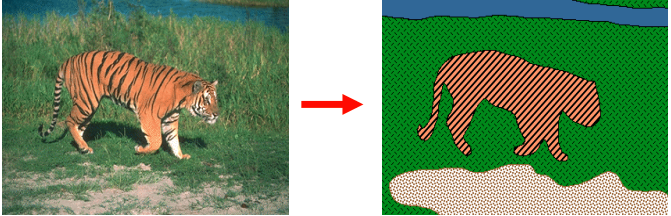
\includegraphics[width=12cm]{7_slide_4}
    \caption{Example of segmentation}
    \label{fig:TigerSeg}
\end{figure}

The type of segmentation in Figure ~\ref{fig:TigerSeg} is what we as humans do naturally. We see the Tiger as separate to the grass. Perhaps we may also see the sandy area as seperate from the grass and so on.

\subsubsection{Examples of grouping in Computer Vision}
\begin{figure}[htp]
    \centering
    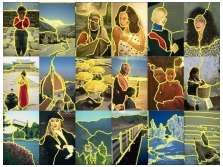
\includegraphics[width=10cm, height=6cm]{slide_5_3}
    \caption{Determining image regions}
    \label{fig:Slide5_3}
\end{figure}

\begin{figure}[htp]
    \centering
    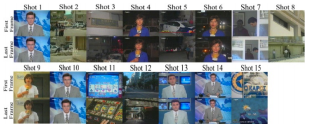
\includegraphics[width=10cm]{slide_5_2}
    \caption{Grouping video frames into shots}
    \label{fig:Slide5_2}
\end{figure}


\begin{figure}[htp]
    \centering
    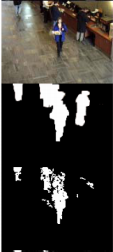
\includegraphics[width=4cm,height=8cm]{slide_5_1}
    \caption{Background Subtraction}
    \label{fig:Slide5_1}
\end{figure}

\begin{figure}[htp]
    \centering
    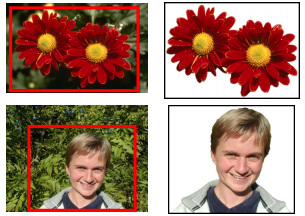
\includegraphics[width=10cm]{slide_5_4}
    \caption{Image segmentation}
    \label{fig:Slide5_4}
\end{figure}

\subsubsection{Basics of grouping in human vision}
As humans we are constantly grouping features together. In a similar way in computer vision we want to group together pixels that \textit{belong together}. The Gestalt school from psychology offers some insight as to how humans group features together.
\subsubsection{The Gestalt School}
The Gestalt school informs us that grouping is key to visual perception. Consider the following image.
\begin{figure}[htp]
    \centering
    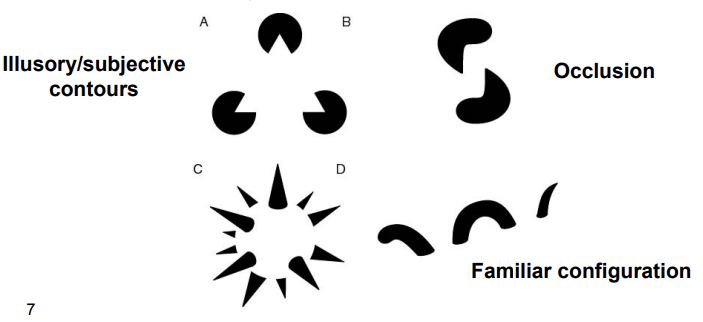
\includegraphics[width=10cm]{slide_7_1}
    \caption{Gestalt School}
    \label{fig:Slide7_1}
\end{figure}

Image A is simply three black circular objects. Despite this our brains can't help but segment these and thus perceive a triangle which isn't actually present. Similar C looks like a sphere despite it simply being black cones.

\subsubsection{Gestalt Factors}
The following are some factors that play into how we group features together.
\begin{figure}[htp]
    \centering
    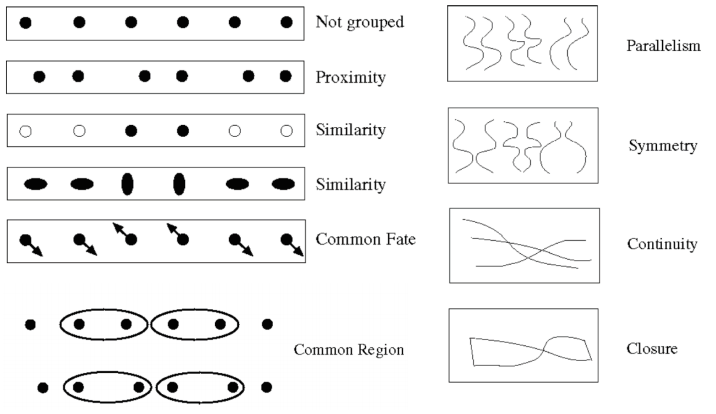
\includegraphics[width=12cm]{slide_8_1}
    \caption{Gestalt Factors}
    \label{fig:Slide8_1}
\end{figure}

\subsubsection{Back to pixels}
Our goal is to group (i.e. segment) pixels. We will do this with the Gestalt factors in mind, however we aren't able to incorporate all of them so we will focus on the simpler factors such as: similarity (pixel values), proximity (pixels close together), etc.
\\\\
Let us define Segmentation more concretely.
\begin{definition}{Segmentation}
\\
Segmentation is the compact representation of image data in terms of a set of \textbf{components}. Components share common \textbf{visual properties} and these properties can be defined at different levels of abstraction.
\end{definition}

\subsubsection{The Goals of Segmentation}
We wish to emphasise that the goal of segmentation is to separate an image into coherent objects. To motivate this, let us consider the following examples of human segmentation.

\begin{figure}[htp]
    \centering
    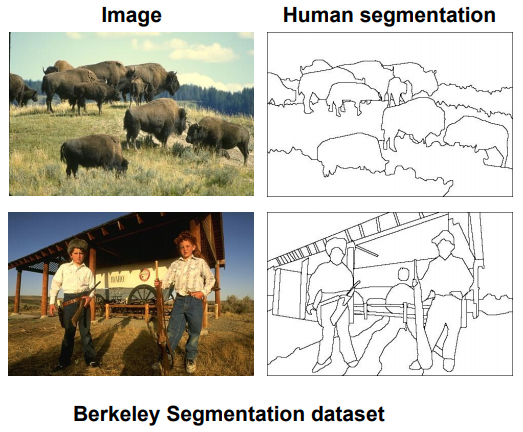
\includegraphics[width=12cm]{slide_10_1}
    \caption{Human segmentation}
    \label{fig:Slide10_1}
\end{figure}

\begin{figure}[htp]
    \centering
    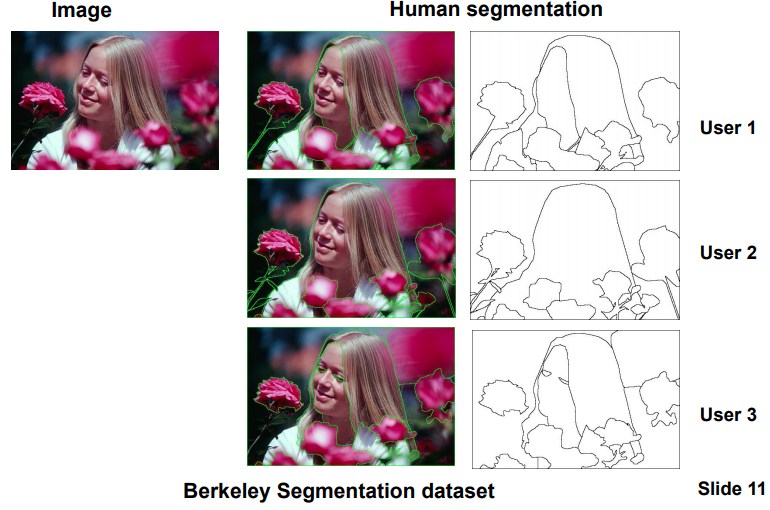
\includegraphics[width=12cm]{slide_11_1}
    \caption{Human segmentation}
    \label{fig:Slide11_1}
\end{figure}

Figure ~\ref{fig:Slide11_1} shows us that humans don't even agree on how to segment an image.
\\\\
Given this knowledge how can we expect a computer to do properly segment an image? It turns out that we don't need a computer to do a perfect human segmentation. The type of segmentation depends on the particular task at hand.

\begin{figure}[htp]
    \centering
    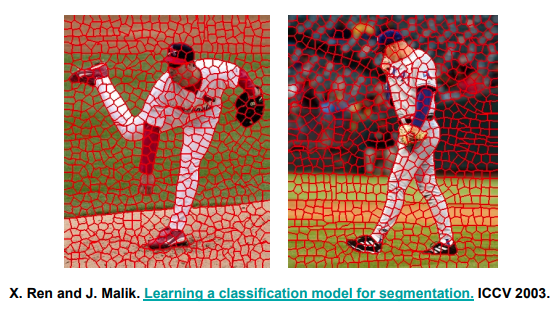
\includegraphics[width=12cm]{slide_12_1}
    \caption{Image segmentation based on similar pixels}
    \label{fig:Slide12_1}
\end{figure}

\newpage
Figure ~\ref{fig:Slide12_1} shows segmentation using super pixels. This helped improve efficiency as rather than considering each and every pixel we can consider regions of super pixels.

\subsection{Segmentation as clustering}
Segmentation can be viewed as a clustering problem as we will see in this section.
\subsubsection{Image Segmentation: Toy Example}
Suppose we have the following input image with no noise (we can generate such an image using a computer).

\begin{figure}[htp]
    \centering
    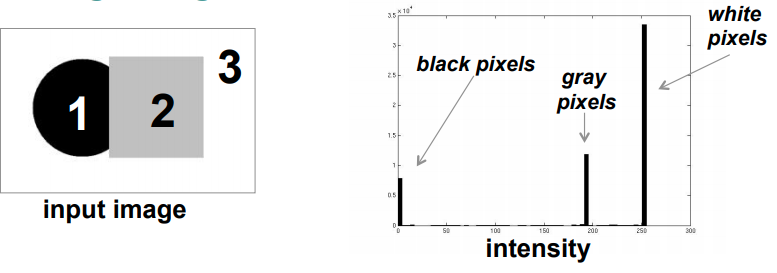
\includegraphics[width=12cm]{slide_14_1}
    \caption{Input image without noise}
    \label{fig:Slide14_1}
\end{figure}

Figure ~\ref{fig:Slide14_1} is trivial to segment. We simply create a histogram of the pixel values and label the peaks. The three discrete peaks in the histogram forms our three groups and so we can label the black circle, the grey square and the white background as required.
\\\\
However this situation is too artificial. We are more likely to have the following variation of the input image with noise.

\begin{figure}[htp]
    \centering
    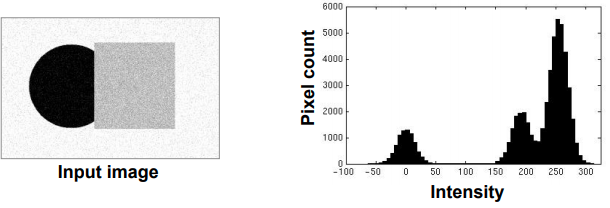
\includegraphics[width=12cm]{slide_16_1}
    \caption{Input image with noise}
    \label{fig:Slide16_1}
\end{figure}

As you can see the histogram isn't as discretised as before. For example the black pixels are now across a certain intensity range, i.e. they vary in terms of how \textbf{black} the pixels are. The same can be said about the white background and the grey square. As a result, in order to segment this new input image we need to \textbf{cluster}.
\\\\
In order to appreciate clustering let us consider the histogram from Figure ~\ref{fig:Slide16_1} in 1 dimension as follows.

\begin{figure}[htp]
    \centering
    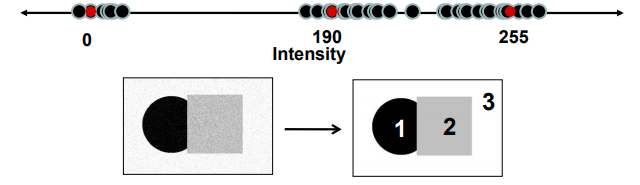
\includegraphics[width=12cm]{slide_17_1}
    \caption{Clustering in 1D}
    \label{fig:Slide17_1}
\end{figure}



Our goal here is to choose three \textbf{centres} from the intensity values to consider as centroids of our clusters. 
\\\\
We then associate pixels to a given cluster based on which centre it is closest to according to the following sum of squared distances (SSD) equation. The \textbf{best cluster centre} is therefore the ones that minimise the SSD between all pixel points, $p$, and a cluster centre, $c_i$.
\begin{equation}
 \Sigma_{p} {\vert\vert p - c_i \vert\vert}^2 \label{eq:SSD}
\end{equation}
\\
This allows us to split our points into three groups as shown in Figure ~\ref{fig:Slide17_1}.
\subsubsection{Clustering}
At this stage we have clusters but we may not have good representatives for each cluster. For example there may be a pixel that is exactly on the boundary between all the other clusters. Since we now know all the pixels that belong to each cluster, we recalculate a new centre for each cluster thanks to the calculations SSD computations we have just carried out.
\\\\
We repeat this process of recalculating a new cluster centre and associating representatives based on Equation \ref{eq:SSD} until we found that the centres stop moving. Thus we arrive at the following clustering solution.

\begin{figure}[htp]
    \centering
    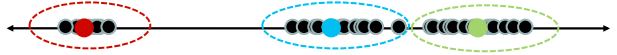
\includegraphics[width=12cm]{slide_18_1}
    \caption{Finished clusters}
    \label{fig:Slide18_1}
\end{figure}

We have so far essentially described the K-Means clustering method. We will now summarise it.

\subsubsection{K-Means Clustering}
Given pixel points that we wish to cluster, we start by arbitrarily initialising $k$ cluster centres. Repeat the process of associating pixels to centres using Equation \ref{eq:SSD} and recalculating new cluster centres. We stop when the cluster centres stop changing. Thus the algorithm proceeds as follows.

\subsubsection*{K-Means Clustering: Algorithm}
\begin{enumerate}
\item Arbitrarily initialise the cluster centres: $c_1, c_2, ..., c_k$.
\item For each pixel point $p$, associate $p$ to a cluster $c_i$ by calculating the sum of squared distances (SSD) (i.e. Equation \ref{eq:SSD}) and associating $p$ to the $c_i$ that yields the minimum SSD. That is, put $p$ in the $i$-th cluster that is closest to it.
\item Recalculate the centres of each cluster, $c_i$, by finding the mean of pixel  points in $c_i$.
\item If $c_i$ has changed, then go to step 2.
\end{enumerate}

\subsubsection*{K-Means Clustering: Properties}
\begin{itemize}
\item K-Means will always converge to \textit{some} solution.
\item The solution may be a local minimum i.e. not the optimal solution for the objective function given by Equation \ref{eq:SSD}.
\end{itemize}

\subsubsection{Feature Space: 1D}
The type of feature space we use dictates the precise way we will group pixels together. Here we are using the familiar 1D feature space that we have been considering so far. In this 1D case we group pixels based on \textbf{colour similarity}. That is we cluster pixels together that are \textit{close} in terms of their brightness or pixel value intensity.

\begin{figure}[htp]
    \centering
    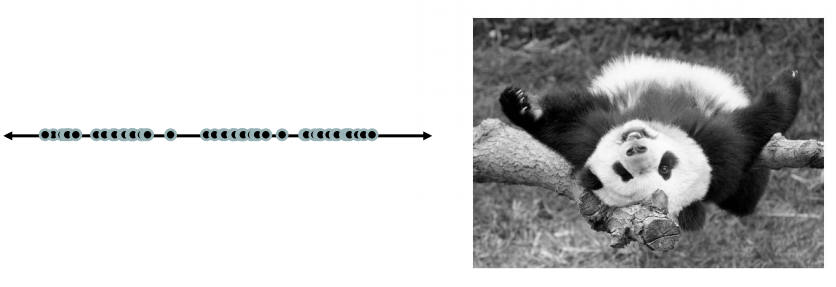
\includegraphics[width=12cm]{slide_20_1}
    \caption{1D Feature space clustering}
    \label{fig:Slide20_1}
\end{figure}

The following shows the results of running K-Means on the image of the panda in Figure \ref{fig:Slide20_1} with $k = 2$ and $k = 3$ clusters. 

\newpage

\begin{figure}[htp]
    \centering
    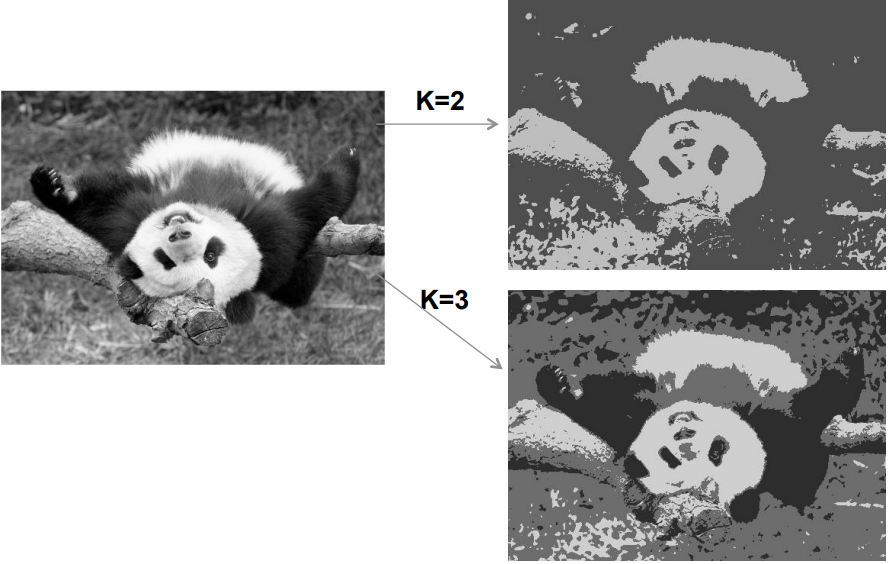
\includegraphics[width=12cm]{slide_21_1}
    \caption{1D Feature space with different clusters.}
    \label{fig:Slide21_1}
\end{figure}

When $k = 2$ we essentially have a binary segmentation since we only have two clusters. We essentially obtain a binary black or white image. However when $k = 3$ when we are able to perhaps segment the image more appropriately.

\subsubsection{Feature Space: 3D}
Suppose we are now trying to run K-Means on an RGB image, our feature space is now actually 3D since we have three colour channels to consider.
\\\\
This time we will group pixels based on \textbf{colour similarity}. For example, pixels that are \textit{blueish} will be grouped together. The following is a demonstration of this in action.

\newpage

\begin{figure}[htp]
    \centering
    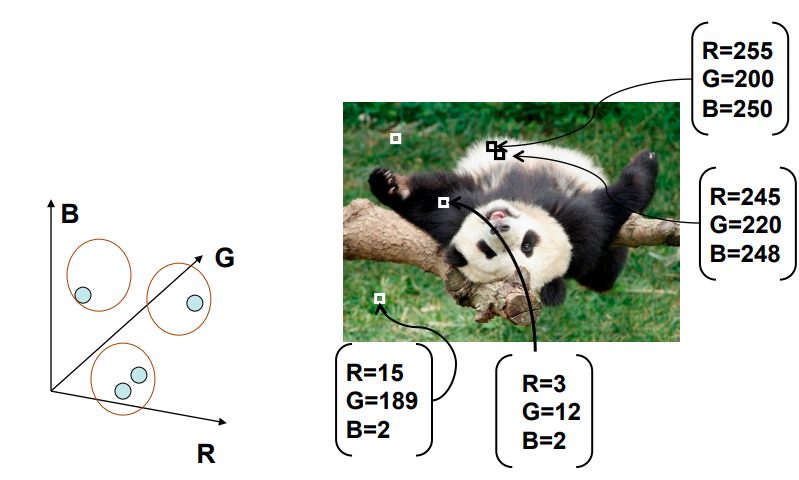
\includegraphics[width=13cm]{slide_22_1}
    \caption{3D Feature space}
    \label{fig:Slide22_1}
\end{figure}

Notice that the limitation with working with only the 3D (r, g, b) feature space is that we cannot segment specific details. For example if we were only interested in the Panda's eyes then using only (r, g, b) would not allow us to adequately cluster in order to only obtain the eyes. To see this, consider the following figure.

\begin{figure}[htp]
    \centering
    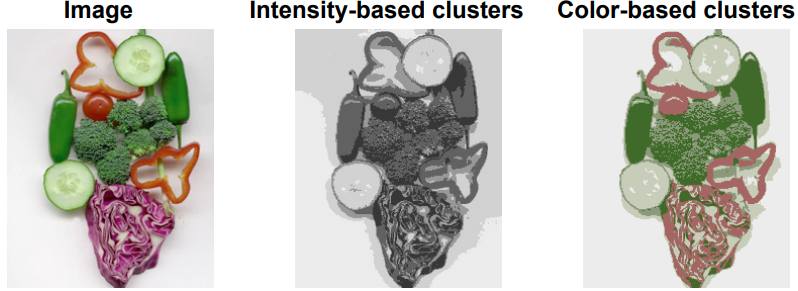
\includegraphics[width=13cm,height=4cm]{slide_23_1}
    \caption{Intensity-based clustering vs Colour-based clustering}
    \label{fig:Slide23_1}
\end{figure}

In Figure \ref{fig:Slide23_1}, the 1D intensity-based feature space and the 3D (r, g, b) colour-based feature space.
\\\\
From this we can observe some problems with the using (r, g, b) feature space. Namely, the clusters that form are \textbf{not spatially coherent}. There are red pappers towards the middle-right, but there is also a red pepper and a red tomato towards the top.
\\\\
For some applications, clustering based on (r, g, b) feature space alone may be desireable however we aren't able to for example pick out the two peppers separately. This is due to the lack of spatial coherence.
\\\\
We can cluster using the 5D (r, g, b, x, y) feature space to enforce spatial coherence. Here (x,y) denotes the position of a pixel point.

\subsubsection{Feature Space: Another 3D feature space}

Let us now consider clustering the Panda image using the 3D (intensity, x, y). We group pixels based on \textbf{intensity and position} similarity.

\begin{figure}[htp]
    \centering
    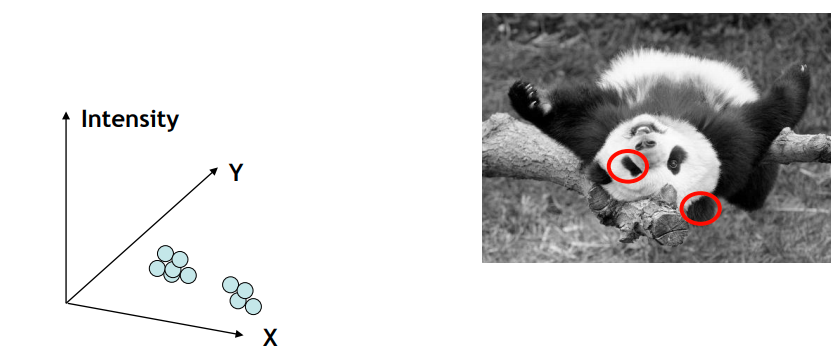
\includegraphics[width=13cm]{slide_24_1}
    \caption{3D (intensity, x, y) feature space}
    \label{fig:Slide24_1}
\end{figure}

Using this feature space, we are able to cluster and pick out specific features such as the eye or ear. Hence we have encoded both similarity and proximity with this feature space.

\subsubsection{K-Means Clustering: Summary}
\subsubsection*{Pros}
\begin{itemize}
\item K-Means Clustering is \textbf{simple and fast} to compute. It is a good starting point for clustering. K-Means is often used as a starting point for a more refined segmentation.

\item K-Means is also guaranteed to converge, albeit only to a local minimum.
\end{itemize}


\subsubsection*{Cons}
\begin{itemize}

\item It often isn't obvious how we should choose the number of clusters, $k$. Although there are algorithms that can help us with this choice.

\item A big problem is that K-Means is very \textbf{sensitive to outliers} as shown in Figure \ref{fig:Slide25_1} below which shows, with (A), K-Means undesirable clusters and, with (B), the ideal clusters we were looking for.

\item \textbf{Converges to a local minimum} so the solution is starting point dependent. As a result we may have to run K-Means with different starting points and then choose the best solution that we get from all the different starting points.

\item K-Means \textbf{detects only spherical clusters}. So if the dataset is not linear, as in Figure \ref{fig:Slide25_2} (B), we get undesirable clusters. This is because of the distance metric that K-Means is using (Equation \ref{eq:SSD}) which is the Euclidean distance. 

From the study of Metric Spaces, we know that the Euclidean metric yields circular neighbourhoods (i.e. \textit{balls}) in 2D and spherical neighbourhoods in 3D.

\item K-Means gives a binary YES/NO answer as to whether a point belongs to a cluster. Often in Computer Vision, we want to work with probabilities (i.e. 67\% chance for class 1, 33\% chance for class 2) so that we can evaluate the uncertainty later on.
\end{itemize}

\begin{figure}[htp]
    \centering
    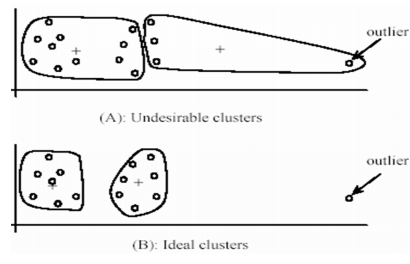
\includegraphics[width=10cm,height=7cm]{slide_25_1}
    \caption{3D (intensity, x, y) feature space}
    \label{fig:Slide25_1}
\end{figure}

\newpage

\begin{figure}[htp]
    \centering
    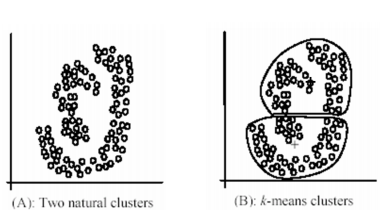
\includegraphics[width=10cm, height=5cm]{slide_25_2}
    \caption{3D (intensity, x, y) feature space}
    \label{fig:Slide25_2}
\end{figure}

\subsection{Probabilistic clustering}
\subsubsection{Motivation}
Probabilistic clustering involves associating a notion of \textit{likelihood} to how we associate a pixel point to a given cluster. As we have seen in the previous section, K-Means completely neglects this notion.
\\\\
Probabilistic clustering addresses the folllowing questions which K-Means does not:
\begin{itemize}
\item What is the probability that a point $p$ is in cluster $m$?
\item What is the shape of each cluster?
\end{itemize}
The idea is to look at the data that we wish to cluster and consider whether the points fit a known continuous function such as the gaussian distribution. 
\\\\
This function is called our \textbf{generative model} since we assume that points in our dataset are generated by sampling this continuous function. The generative model is defined by a \textbf{vector of parameters}, $\theta$, which encodes values such as position and mean.

\subsubsection{Mixture of Gaussians}
We will now consider the Mixture of Gaussians (MoG) method for probabilistic clustering. However, we will first need the following definition.

\begin{definition}{Covariance}
\\
Let x and y be vectors of length n.
\\\\
Then the covariance of x and y is given by, cov(x, y) = $\Sigma_{i=1}^{n} {\frac{(x_i - \bar{x})(y_i - \bar{y})}{n}}$
\end{definition}

\begin{remark}
Covariance provides a measure of the strength of the correlation between two or more sets of random variates.
\end{remark}
\noindent This leads nicely to the following definition.

\begin{definition}{Covariance Matrix}
\\
Let $x=(x_1, ..., x_n)$ be a vector of length n.
\\\\
Then the covariance matrix, denoted by $\Sigma$, for $x$ is an $N \times N$ matrix that gives the covariance between each pair of elements of $x$. $\Sigma$ is given by,
\\\\
$
\Sigma = \begin{bmatrix}
cov(x_1,x_1) & \cdots & cov(x_1, x_n)\\
\vdots & \ddots & \vdots\\
cov(x_n, x_1) & \cdots & cov(x_n, x_n)
\end{bmatrix}
$
\end{definition}

\begin{remark}
The diagonal entries in the covariance matrix is the variance.
\end{remark}

\noindent The Mixture of Gaussians (MoG) is a generative model for clustering. We can use MoG in the following situaiton.

\begin{figure}[htp]
    \centering
    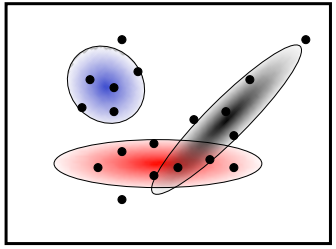
\includegraphics[width=8cm, height=5cm]{slide_29_1}
    \caption{Mixture of Gaussians}
    \label{fig:Slide29_1}
\end{figure}

\noindent Notice that the black points more or less follow a gaussian distribution. Hence we use the gaussian distribution as a model for generating each cluster. This results in us forming the three clusters as seen in Figure \ref{fig:Slide29_1}.

\subsubsection*{Computing the Gaussian Mixture}

Let $x = (x_1, ..., x_d)$ be a vector of length $d$. We associate a blob, $b$, to a cluster $k$ based on the following multivariate gaussian probability distribution:

\begin{equation}
P(x \vert \mu_b, \Sigma_b) = \frac{1}{\sqrt{(2\pi)^{d}det(\Sigma)}}e^{ -\frac{1}{2}(x - \mu_b)^{\top}\Sigma^{-1}(x - \mu_b)}
\end{equation}

\noindent Here $\mu_b$ denotes the mean of points in the blob $b$ and $\Sigma_b$ denotes the covariance matrix for the points in $b$.
\\\\
The \textbf{likelihood} of observing the point $x$ is given by a weighted mixture of gaussians as follows,
\begin{equation}
P(x \vert \theta) = \Sigma_{b=1}^k \alpha_{b}P(x \vert \theta_b), \text{where} \: \theta = [\mu_1, ..., \mu_d, \Sigma_1, ..., \Sigma_b]
\end{equation}

\subsubsection{Expectation Maximisation (EM)}










\end{document}


